\documentclass[pdflatex,11pt]{../aghdoc_version2}
% \documentclass{../aghdoc}               % przy kompilacji programem latex
\usepackage[polish]{babel}
\usepackage[utf8]{inputenc}

% dodatkowe pakiety
\usepackage{enumerate}
\usepackage{listings}
\usepackage{caption}

% żeby stopki były zastosowane do stron gdzie rozpoczyna się rozdział
\usepackage{etoolbox}
\patchcmd{\chapter}{\thispagestyle{plain}}{\thispagestyle{fancy}}{}{}

\lstloadlanguages{TeX}

\lstset{
  literate={ą}{{\k{a}}}1
           {ć}{{\'c}}1
           {ę}{{\k{e}}}1
           {ó}{{\'o}}1
           {ń}{{\'n}}1
           {ł}{{\l{}}}1
           {ś}{{\'s}}1
           {ź}{{\'z}}1
           {ż}{{\.z}}1
           {Ą}{{\k{A}}}1
           {Ć}{{\'C}}1
           {Ę}{{\k{E}}}1
           {Ó}{{\'O}}1
           {Ń}{{\'N}}1
           {Ł}{{\L{}}}1
           {Ś}{{\'S}}1
           {Ź}{{\'Z}}1
           {Ż}{{\.Z}}1
}

%---------------------------------------------------------------------------

\author{Tomasz Kasprzyk, Daniel Ogiela, Jakub Stępak}
\shortauthor{T. Kasprzyk, D. Ogiela, J.Stępak}

\titlePL{System obliczający wyniki wyborów dla uogólnienia systemu k-Borda}

\shorttitlePL{System obliczający wyniki wyborów dla uogólnienia systemu k-Borda} % skrócona wersja tytułu jeśli jest bardzo długi

\thesistypePL{Dokumentacja techniczna}

\supervisorPL{dr hab. inż. Piotr Faliszewski}

\date{2016}

\departmentPL{Katedra Informatyki}

\facultyPL{Wydział Informatyki, Elektroniki i Telekomunikacji}

\setlength{\cftsecnumwidth}{10mm}

% umożliwienie żeby domyślnie dokument nie robił wcięć poza wybranymi (\indent w tym miejscu)

\newlength\tindent
\setlength{\tindent}{\parindent}
\setlength{\parindent}{0pt}
\renewcommand{\indent}{\hspace*{\tindent}}

\fancypagestyle{plain}{%
\fancyhf{} % clear all header and footer fields
\fancyhead[R]{\bfseries \thepage}
\fancyfoot[C]{System obliczający wyniki wyborów dla uogólnienia systemu k-Borda} % except the center
\renewcommand{\headrulewidth}{0.5pt}
\renewcommand{\footrulewidth}{0.5pt}}

%---------------------------------------------------------------------------

\begin{document}

\titlepages

\tableofcontents\thispagestyle{fancy}


%----------------------------------------------------------------------------
\chapter{Dziedzina problemu}
\label{cha:dziedzina_problemu}

\section{Metoda obliczania wyników wyborów}
\label{sec:metoda_obliczania_wynikow_wyborow}

\subsection{Metoda Bordy}
\label{subsec:metoda_bordy}

Niech $v$ będzie głosem nad zbiorem kandydatów $C$. Wynik według Bordy kandydata $c$ w $v$ jest równy $\beta(i)=C-i$, gdzie $i$- pozycja kandydata w ciągu $v$.
Wynik $c$ w wyborach jest sumą wyników $c$ u każdego z wyborców


\subsection{Metoda k-Borda}
\label{subsec:metoda_k_borda}

Rozszerzenie metody Bordy. Wynik, zamiast dla jednego kandydata, obliczany jest dla ciągu kandydatów. $f_{kB}$- funkcja zadowolenia z komitetu. Ciąg $(i_1,\dots, i_k)$- ciąg pozycji kandydatów

\paragraph{Przyklad}
$C={c_1,c_2,c_3,c_4}$ - zbiór kandydatów, 
$v=(c_2,c_1,c_4,c_3)$ - głos
Niech $k = 2$ (wybory $2$ spośród $4$)
$w=(c_4,c_3)$
Najpierw określamy pozycje kandydatów z komitetu $w$ w $v$:
$pos_v(w)=(3,4)$, zatem wynik komitetu w dla głosu v wynosi
$f_{kB}(3,4) = (3) + (4) = ||C|| - 3 ) + ( ||C|| - 4 ) = 1 + 0 = 1$


\subsection{Uogólnienie - system $\ell_p$ Borda}
\label{subsec:system_ell_p_borda}

Zanim wprowadzone zostanie pojęcie uogólnionego systemu k-Borda warto przypomnieć wzór na normę $\ell_p$

\subsubsection{Norma $\ell_p$}
\label{subsubsection:norma_ell_p}

$\ell_p(x_1,x_2,\dots, x_n) = \sqrt[p]{x_1^p+x_2^p+\dots+x_n^p},$ 


Wówczas, w uogólnionej wersji metody k-Borda, funkcja zadowolenia $f_{kB}$ zostaje uzależniona również od parametru $p$ z powyższego wzoru. Norma liczona jest z wyników według Bordy, $\beta(i)$. Wzór uogólniony funkcji zadowolenia przyjmuje zatem postać:\\
$f_{\ell_pB}(p,(i_11,\dots,i_k))=p[(i1)]p+[(i2)]p+...+[(ik)]p$


Systemy  k-Borda i Cahmberlin’a-Courant’a są szczególnymi przypadkami zdefiniowanego powyżej systemu $\ell_p$- Borda:\\
Dla $p = 1$, $l_1$\\
$f_{\ell_pB}(1,(i_1, \dots ,i_k)) = \beta(i_1) + \beta(i_2) + \dots + \beta(ik) = f_{kB}(i_11, \dots,i_k)$\\
Dla $p= \infty$,  $l_{\infty}={max}$\\
$f_{\ell_pB}(\infty,(i_1, \dots ,i_k))=\lim\limits_{p \to \infty} \sqrt[p]{\beta\left[(i_1)\right]^p+\beta\left[(i_2)\right]^p+ \dots +\left[\beta(i_k)\right]^p}=\max{\beta(i_1),\beta(i_2),\dots,\beta(i_k)} = \beta(i_1)=f_{CC}$

\section{Format danych wejściowych}
\label{sec:format_danych_wejsciowych}
Pojedynczy plik składa się z następującego formatu:\\
\texttt{<liczba kandydatów> \\
1, <nazwa kandydata> \\
2, <nazwa kandydata> \\
… \\
<liczba kandydatów>, <nazwa kandydata> \\
<liczba głosujących>, <liczba głosów policzonych>, <liczba unikalnych głosów> \\
<liczba powtórzeń głosu>, <głos> \\
… \\
<liczba powtórzeń głosu>, <głos>}

\chapter{Architektura Django}
$Django$ to framework webowy napisany w $Pythonie$. Dostarcza wysokopoziomowych
abstrakcji pozwalających na szybkie i wygodne pisanie przejrzystych aplikacji. \\ \\
Jego architektura koncepcyjnie przypomina wzorzec architektoniczny $Model-View-Controller$,
jednak jak przyznają sami twórcy [ref], $Django$ nie do końca wpasowuje się w klasyczne
ujęcie $MVC$. \\ \\
$Django$ dostarcza mapowania obiekto-relacyjnego, dzięki którym całość modeli można ująć
w $Pythonie$. Wygodny $ORM$ zazwyczaj wystarcza do obsługi bazy danych, jednak zawsze
istnieje możliwość użycia bezpośrednio $SQL$. \\ \\
Widoki w $Django$ spełniają dwojaką funkcję - służą zarówno przekazaniu danych do
wyświetlenia, jak i ich modyfikacji. W wyświetleniu danych użytkownikowi pośredniczą
szablony ($templates$), które "opakowują" przekazane dane do postaci $HTMLa$, który może
wyświetlić przeglądarka internetowa. Dzięki temu wybór danych, jakie mają zostać pokazane
użytkownikowi jest oddzielony od samego sposobu ich prezentacji. \\ \\
Za kontroler z klasycznego $MVC$ można uznać sam framework dostarczający wspomnianej
obsługi bazy danych czy mapowania adresów URL do poszczególnych widoków.

\chapter{Opis modułów}
\label{cha:opis_modulow}

\section{Moduł administracji kont}
\subsection{Opis ogólny}
Moduł odpowiedzialny za zarządzanie kontami użytkowników. Umożliwia czynności
logowania, wylogowania oraz rejestracji. Nie współpracuje z innymi modułami. Korzysta
jedynie z bazy danych w celu weryfikacji użytkowników.

\subsection{Komponenty programowe}
Komponenty programowe dla tego modułu znajdują się w pakiecie $ecs.accounts$ \\ \\
{
\centering
\begin{tabular}{|c|c|c|}
\hline 
\textbf{Typ komponentu} & \textbf{Komponenty} & \textbf{Wykorzystanie} \\ 
\hline 
widoki & klasa $LoginView$ & logowanie \\ 
\cline{2-3} 
 & klasa $RegisterView$ & rejestracja \\ 
\hline 
szablony & $login.html$ & logowanie \\ 
\cline{2-3} 
 & $register.html$ & rejestracja \\ 
\hline 
formularze & klasa $LoginForm$ & logowanie \\ 
\cline{2-3} 
 & klasa $RegistrationForm$ & rejestracja \\ 
\hline 
\end{tabular} 
}

\section{Moduł zarządzania wyborami}
\subsection{Opis ogólny}
Moduł odpowiedzialny za administrację wyborami i ich wynikami. Umożliwia podstawowe
operacje na wyborach i ich wynikach oraz nawigację między nimi. Pozwala na wyświetlenie
listy wszystkich wyborów i ich wyników, stworzenie nowych wyborów lub wyniku, czy
usunięcie wyborów. W celu wykonania niektórych zadań współpracuje z modułem obliczania
wyników wyborów oraz modułem wizualizacji wyborów i ich wyników. Jest to najbardziej
rozbudowany moduł.

\subsection{Komponenty programowe}
% \usepackage{array} is required
\begin{tabular}{|c|c|p{5cm}|}
\hline 
\textbf{Typ komponentu} & \textbf{Komponenty} & \textbf{Wykorzystanie} \\ 
\hline 
widoki & klasa $ElectionListView$ & wyświetlenie listy wszystkich wyborów \\ 
\cline{2-3} 
 & klasa $ElectionCreateView$ & stworzenie wyborów \\ 
\cline{2-3} 
 & klasa $ElectionDeleteView$ & usunięcie wyborów \\ 
\cline{2-3} 
 & klasa $ElectionDetailView$ & wyświetlenie informacji szczegółowych o
danych wyborach \\ 
\cline{2-3} 
 & klasa $ResultCreateView$ & stworzenie wyniku dla danych wyborów -
wyświetlenie formularza określającego
parametry wyniku \\ 
\cline{2-3} 
 & klasa $ResultDetailsView$ & wyświetlenie danego wyniku danych
wyborów \\ 
\cline{2-3} 
 & klasa $ResultDeleteView$ & usuwanie pojedynczego wyniku wyborów \\ 
\hline 
szablony & $election_list.html$ & wyświetlenie listy wszystkich wyborów,
usunięcie wyborów - strona sukcesu
wyświetlana po usunięciu wyborów \\ 
\cline{2-3} 
 & $election_create.html$ & stworzenie wyborów \\ 
\cline{2-3} 
 & $election_details.html$ & stworzenie wyborów - strona sukcesu
wyświetlana po stworzeniu wyborów,
wyświetlenie informacji szczegółowych o
danych wyborach \\ 
\cline{2-3} 
 & $election_delete.html$ & usunięcie wyborów \\ 
\cline{2-3} 
 & $result_create.html$ & stworzenie nowego wyniku wyborów -
strona z formularzem \\ 
\cline{2-3} 
 & $result_details.html$ & wyświetlenie danego wyniku danych
wyborów \\ 
\cline{2-3} 
 & $result_delete.html$ & potwierdzenie usunięcia rezultatu \\ 
\hline 
formularze & klasa $ElectionForm$ & stworzenie wyborów \\ 
\cline{2-3}
 & klasa $ResultForm$ & stworzenie wyniku dla danych wyborów -
formularz określający parametry wyniku \\
\hline 
\end{tabular} 

\section{Moduł wizualizacji wyborów i wyników wyborów}
\subsection{Opis ogólny}
Moduł odpowiedzialny za stworzenie wykresu $2D$ wizualizującego wybory i jego wyniki.
Wizualizacja dotyczy tylko wyborów wygenerowanych z rozkładu normalnego. Wyborcy i
kandydaci są reprezentowani jako punkty na płaszczyźnie. Punkty reprezentujące wyborców
i kandydatów mają na wykresie odmienne kolory. Na wykresie wyników wyborów punkty
reprezentujące zwycięzców wyborów są powiększone. Moduł współpracuje z modułem
zarządzania wyborów, który zleca mu zadanie wizualizacji wyborów lub jego wyników. W
celu wykonania zadania moduł wizualizacji wyborów i wyników wyborów pobiera dane z
bazy danych.

\subsection{Komponenty programowe}
\begin{tabular}{|c|c|p{5cm}|}
\hline 
\textbf{Typ komponentu} & \textbf{Komponenty} & \textbf{Wykorzystanie} \\ 
\hline 
widoki & klasa $ScatterChartMixin$ & pobranie danych potrzebnych do
wygenerowania wykresów (punkty, tytuł
wykresu, serii danych), dziedziczy po
klasie $View$ \\ 
\cline{2-3} 
 & klasa $ElectionChartView$ & wizualizacja wyborów, klasa dziedziczy
po klasie $ScatterChartMixin$, pobranie
współrzędnych kandydatów i wyborców \\ 
\cline{2-3} 
 & klasa $ResultChartView$ & wizualizacja wyników wyborów, klasa
dziedziczy po klasie $ScatterChartMixin$,
pobranie współrzędnych kandydatów,
wyborców oraz zwycięzców \\ 
\hline 
\end{tabular} 

\section{Moduł generacji i wczytywania wyborów}
\subsection{Opis ogólny}
Moduł odpowiedzialny za generację wyborów z rozkładu normalnego oraz wczytywanie
wyborów z pliku formatu $.soc$. Moduł współpracuje z modułem zarządzania wyborami,
któremu zleca po wykonaniu swoich zadań, stworzenie i wysłanie użytkownikowi
odpowiedniej strony internetowej. Moduł zapewnia wygenerowanie wyborów z rozkładu normalnego według wskazanych parametrów oraz walidację danych przy wczytywaniu
wyborów z pliku. Po stworzeniu wyborów moduł komunikuje się z bazą danych w celu
utrwalenia wyborów.

\subsection{Komponenty programowe}
\begin{tabular}{|c|c|p{5cm}|}
\hline 
\textbf{Typ komponentu} & \textbf{Komponenty} & \textbf{Wykorzystanie} \\ 
\hline 
Widoki & klasa $ElectionLoadDataFormView$ & wczytanie wyborów z pliku \\ 
\cline{2-3} 
 & klasa
$ElectionGenerateDataFormView$ & generacja wyborów z rozkładu
normalnego \\ 
\hline 
Szablony & $election_load_data.html$ & strona z formularzem do
wskazania pliku \\ 
\cline{2-3} 
 & $election_generate_data.html$ & strona z formularzem do
wskazania parametrów wyborów i
rozkładu normalnego \\ 
\cline{2-3} 
 & $election_details.html$ & strona wyświetlana po
poprawnym wczytaniu danych z
pliku \\ 
\hline 
Formularze & klasa $ElectionLoadDataForm$ & wczytanie z pliku \\ 
\hline 
\end{tabular} 

\section{Moduł obliczania wyników wyborów}
\subsection{Opis ogólny}
Moduł odpowiedzialny za obliczanie wyników wyborów. Zapewnia różne algorytmy do
wykonania zadania. Użytkownik ma wybór między algorytmem genetycznym, dwoma
algorytmami zachłannymi oraz algorytmem typu brute-force. Moduł współpracuje z modułem
zarządzania wyborami, który zleca mu wykonanie zadania.
\subsection{Komponenty programowe}
Wszystkie komponenty programowe dotyczące modułu obliczania wyników wyborów
zawierają się w pakiecie $ecs.elections.algorithms$. \\
Klasy odpowiedzialne za poszczególne algorytmy:
\begin{itemize}
\item $BruteForce$ - odpowiedzialna za algorytm typu brute-force
\item $GreedyAlgorithm$ - odpowiedzialna za algorytm zachłanny zależny od parametru $p$
\item $GreedyCC$ - odpowiedzialna za algorytm zachłanny niezależny od parametru $p$
\item $GeneticAlgorithm$ - odpowiedzialna za algorytm genetyczny
\end{itemize}

\section{Moduł URL Resolver}
\subsection{Opis ogólny}
Moduł odpowiedzialny za przekazywanie żądań otrzymywanych przez klienta do
odpowiednich modułów.

\subsection{Komponenty programowe}
Przyporządkowania żądań użytkownika do odpowiednich modułów (adresów URL do
widoków) znajdują się w pliku $ecs.elections.urls.py$.

\chapter{Współpraca modułów i innych komponentów}
\section{Diagram komunikacji}
\begin{center}
\centerline{\includegraphics[scale=0.65]{pics/Diagram_Komunikacji.png}}
\captionof{figure}{Diagram komunikacji}
\end{center}

\section{Ścieżki przejść}
\subsection{Logowanie}
\begin{enumerate}
\item Użytkownik za pomocą przeglądarki internetowej wysyła żądanie logowania.
\item Moduł URL Resolver kieruje żądanie do modułu administracji kont.
\item Moduł administracji kont przesyła do przeglądarki stronę z formularzem do
zalogowania (pole $Username$ i $Password$).
\item Użytkownik wypełnia formularz i za pomocą przeglądarki internetowej wysyła
uzupełniony formularz.
\item Moduł URL Resolver przekazuje żądanie do modułu administracji kont.
\item Moduł administracji kont przeprowadza uwierzytelnienie użytkownika.
\item W zależności od rezultatu uwierzytelnienia podjęte są trzy możliwe akcje:
	\begin{itemize}
	\item jeżeli uwierzytelnienie powiodło się, Moduł administracji kont loguje użytkownika 		i wysyła do
	przeglądarki stronę z wiadomością o sukcesie logowania
	\item jeżeli podana nazwa użytkownika nie istnieje w bazie, Moduł administracji kont 			wysyła do
	przeglądarki internetowej stronę z formularzem do zalogowania (pole
	$Username$ i $Password$) i z informacją o nieistnieniu podanej nazwy
	użytkownika. Następuje przejście do kroku nr $4$
	\item jeżeli podana nazwa użytkownika istnieje w bazie, ale podane hasło jest
nieprawidłowe, Moduł administracji kont wysyła do przeglądarki internetowej stronę z
formularzem do zalogowania (pole $Username$ i $Password$) i z informacją o
błędnym haśle. Następuje przejście do kroku nr $4$
	\end{itemize}
\end{enumerate}

\subsection{Wylogowanie}
\begin{enumerate}
\item Użytkownik za pomocą przeglądarki internetowej wysyła żądanie wylogowania.
\item Moduł URL Resolver kieruje żądanie do modułu administracji kont.
\item Moduł administracji kont wylogowuje użytkownika i przesyła do przeglądarki stronę
domową aplikacji.
\end{enumerate}

\subsection{Rejestracja}
\begin{enumerate}
\item Użytkownik za pomocą przeglądarki internetowej wysyła żądanie zarejestrowania
użytkownika.
\item Moduł URL Resolver kieruje żądanie do modułu administracji kont.
\item Moduł administracji kont przesyła do przeglądarki stronę z formularzem do rejestracji
(pola $E-mail$, $Username$, $Password$, $First name$ i $Last name$).
\item Użytkownik wypełnia formularz i za pomocą przeglądarki internetowej wysyła
uzupełniony formularz.
\item Moduł URL Resolver przekazuje żądanie do modułu administracji kont.
\item Moduł administracji kont przeprowadza walidację danych.
\item W zależności od rezultatu walidacji:
	\begin{itemize}
	\item jeżeli się powiodła, Moduł administracji kont tworzy konto nowego użytkownika, 			zapisuje je do
	bazy danych, loguje użytkownika do nowo utworzonego konta i przesyła do
	przeglądarki stronę z wiadomością o sukcesie logowania
	\item w przeciwnym wypadku, zostaje wysłana do przeglądarki strona z
	formularzem do rejestracji wraz z informacją o znalezionym problemie.
	Następuje przejście do kroku nr $4$
	\end{itemize}
\end{enumerate}

\subsection{Wyświetlenie listy wszystkich wyborów}
\begin{enumerate}
\item Użytkownik klikając przycisk $Your elections$ na stronie, wysyła za pomocą
przeglądarki internetowej żądanie wyświetlenia listy swoich wyborów.
\item Moduł URL Resolver kieruje żądanie do modułu zarządzania wyborami (widok
$ElectionListView$).
\item Moduł zarządzania wyborami kieruje zapytanie do bazy danych o obiekty
reprezentujące wybory danego użytkownika.
\item Po pobraniu z bazy potrzebnych danych moduł zarządzania wyborami za pomocą
szablonu $election\_list.html$ tworzy stronę i wysyła do przeglądarki internetowej
użytkownika.
\end{enumerate}

\subsection{Stworzenie wyborów}
\begin{enumerate}
\item Użytkownik klikając przycisk $New election$ na stronie, wysyła za pomocą
przeglądarki internetowej żądanie stworzenie nowych wyborów.
\item Moduł URL Resolver kieruje żądanie do modułu zarządzania wyborami (widok
$ElectionCreateView$).
\item Widok posiada zdefiniowany szablon $election\_create.html$ i formularz $ElectionForm$.
Wykorzystując te komponenty tworzy i wysyła do użytkownika stronę z formularzem.
\item Użytkownik wypełnia formularz (pola $Name$ i $Commitee size$) i wysyła uzupełniony
formularz.
\item Moduł URL Resolver kieruje żądanie do modułu zarządzania wyborami (widok
$ElectionCreateView$).
\item Widok wykorzystując klasę formularza pobiera dane z formularza, tworzy nowy
obiekt wyborów i zapisuje go do bazy.
\item Widok wykorzystując szablon $election\_details.html$ tworzy stronę i wysyła ją do
przeglądarki użytkownika.
\end{enumerate}

\subsection{Usunięcie wyborów}
\begin{enumerate}
\item Użytkownik klikając ikonę kosza na stronie, wysyła za pomocą przeglądarki
internetowej żądanie usunięcia wyborów.
\item Moduł URL Resolver kieruje żądanie do modułu zarządzania wyborami (widok
$ElectionDeleteView$).
\item Widok posiada zdefiniowany szablon $election\_delete.html$, który wykorzystuje do
stworzenia i wysłania strony potwierdzającej akcję użytkownika.
\item Użytkownik potwierdza chęć usunięcia wyborów przez naciśnięcie przycisku $Yes,
delete this.$ (W przypadku wyboru przycisku $No, cancel$ akcja nie zostaje przeprowadzona a użytkownik zostaje przeniesiony na stronę z listą swoich
wyborów).
\item Moduł URL Resolver kieruje żądanie do modułu zarządzania wyborami (widok
$ElectionDeleteView$).
\item Widok usuwa wybory z bazy danych i wykorzystując szablon $election\_list.html$ tworzy
i wysyła stronę do przeglądarki internetowej użytkownika.
\end{enumerate}

\subsection{Wyświetlenie informacji szczegółowych dla danych wyborów}
\begin{enumerate}
\item Użytkownik klikając na link wyborów na stronie z listą swoich wyborów, wysyła za
pomocą przeglądarki internetowej żądanie wyświetlenia informacji szczegółowych
dla danych wyborów.
\item Moduł URL Resolver kieruje żądanie do modułu zarządzania wyborami (widok
$ElectionDetailView$).
\item Widok pobiera z bazy danych listę głosujących oraz listę wyników wyborów.
\item Jeżeli wybory zostały wygenerowane z rozkładu normalnego, widok przekierowuje
działanie programu do modułu wizualizacji wyborów i wyników wyborów (widok
$ElectionChartView$). Jeżeli wybory nie zostały wygenerowane z rozkładu normalnego, następuje przejście do kroku nr $6$
\item Widok pobiera z bazy danych obiekty będące punktami $2D$ reprezentującymi
wyborców i kandydatów. Ustawia parametry wykresu a następnie wysyła wszystkie
dane z powrotem do widoku $ElectionDetailView$ umożliwiając stworzenie wykresu.
\item Widok wykorzystując szablon $election\_details.html$ tworzy i wysyła stronę do
przeglądarki użytkownika.
\end{enumerate}

\subsection{Stworzenie nowego wyniku dla danych wyborów}
\begin{enumerate}
\item Użytkownik klikając na link $Add new result$ na stronie ze szczegółowymi informacjami
o danych wyborach, wysyła za pomocą przeglądarki internetowej żądanie stworzenia
nowego wyniku dla danych wyborów.
\item Moduł URL Resolver kieruje żądanie do modułu zarządzania wyborami (widok
$ResultCreateView$).
\item Widok wykorzystując formularz $ResultForm$ i szablon $result\_create.html$ tworzy oraz
wysyła do użytkownika stronę z formularzem do określenia parametrów wyniku (pola:
parametr $p$ do obliczania normy oraz typ algorytmu).
\item Użytkownik wypełnia formularz i wysyła go do systemu.
\item Moduł URL Resolver kieruje żądanie do modułu zarządzania wyborami (widok
$ResultCreateView$).
\item Widok wczytuje dane z formularza, pobiera z bazy danych obiekt reprezentujący
wybory a następnie przekierowuje działanie programu do modułu obliczania wyników
wyborów przekazując konieczne parametry.
\item Moduł obliczania wyników wyborów liczy zwycięzców wyborów za pomocą
odpowiedniego algorytmu. Następnie przekazuje sterowanie z powrotem do widoku
$ResultCreateView$ przekazując wyniki.
\item Widok zapisuje wynik do bazy danych i przechodzi do ścieżki \textit{Wyświetlenie
informacji szczegółowych dla danych wyborów}.
\end{enumerate}

\subsection{Wyświetlenie szczegółowych informacji o danym wyniku danych
wyborów}
\begin{enumerate}
\item Użytkownik klikając na link danego wyniku wyborów na stronie ze szczegółowymi
informacjami o danych wyborach, wysyła za pomocą przeglądarki internetowej
żądanie wyświetlenia szczegółowych informacji o danym wyniku dla danych
wyborów.
\item Moduł URL Resolver kieruje żądanie do modułu zarządzania wyborami (widok
$ResultDetailsView$).
\item Widok pobiera z bazy danych informacje o zwycięzcach danych wyborów.
\item Jeżeli wybory zostały wygenerowane z rozkładu normalnego, widok przekierowuje
działanie programu do modułu wizualizacji wyborów i wyników wyborów (widok
$ResultChartView$). Jeżeli wybory nie zostały wygenerowane z rozkładu normalnego, następuje przejście do kroku nr $6$
\item Widok pobiera z bazy danych obiekty będące punktami $2D$ reprezentującymi
wyborców, kandydatów i zwycięzców. Ustawia parametry wykresu a następnie
wysyła wszystkie dane z powrotem do widoku $ResultDetailsView$ umożliwiając
stworzenie wykresu.
\item Widok wykorzystując szablon $result\_details.html$ tworzy i wysyła stronę do
przeglądarki użytkownika.
\end{enumerate}

\subsection{Wczytanie wyborów z pliku .soc}
\begin{enumerate}
\item Użytkownik klikając na przycisk $Load data from file$ na stronie ze szczegółowymi
informacjami o danych wyborach, wysyła za pomocą przeglądarki internetowej
żądanie wczytania wyborów z pliku $.soc$.
\item Moduł URL Resolver kieruje żądanie do modułu generacji i wczytywania wyborów (widok
$ElectionLoadDataFormView$).
\item Widok wykorzystując formularz $ElectionLoadDataForm$ i szablon
$election_load_data.html$ tworzy oraz wysyła do użytkownika stronę z formularzem do
wybrania pliku, z którego będą wczytywane wybory.
\item Użytkownik wskazuje plik i wysyła uzupełniony formularz do systemu.
\item Moduł URL Resolver kieruje żądanie do modułu generacji i wczytywania wyborów (widok
$ElectionLoadDataFormView$).
\item Widok parsuje plik wejściowy i waliduje dane. W przypadku poprawnego wczytania
pliku wejściowego następuje zapis wczytanych obiektów do bazy danych. Za pomocą
szablonu $election\_details.html$ zostaje stworzona i wysłana strona do przeglądarki
użytkownika.
\end{enumerate}

\subsection{Generacja wyborów z rozkładu normalnego}
\begin{enumerate}
\item Użytkownik klikając na przycisk $Generate election from normal distribution$ na stronie
ze szczegółowymi informacjami o danych wyborach, wysyła za pomocą przeglądarki
internetowej żądanie wygenerowania wyborów za pomocą rozkładu normalnego.
\item Moduł URL Resolver kieruje żądanie do modułu generacji i wczytywania wyborów (widok
$ElectionGenerateDataFormView$).
\item Widok wykorzystując formularz $ElectionGenerateDataForm$ i szablon
$election\_generate\_data.html$ tworzy oraz wysyła do użytkownika stronę z formularzem do
określenia parametrów wyborów oraz i rozkładu normalnego.  
\item Użytkownik uzupełnia formularz i wysyła go do systemu.
\item Moduł URL Resolver kieruje żądanie do modułu generacji i wczytywania wyborów (widok
$ElectionGenerateDataFormView$).
\item Widok wczytuje dane z formularza i wykorzystując generator, generuje według
wczytanych parametrów kandydatów, wyborców oraz liczy ich preferencje. Dane
zostają zapisane do bazy. Następnie program przechodzi do 2-go punktu ścieżki
\textit{Wyświetlanie informacji szczegółowych dla danych wyborów}.
\end{enumerate}

\chapter{Struktura obiektowa przechowywanych danych}
\section{Opis modeli wykorzystywanych w ORM}
Poniżej zamieszczono opis klas wykorzystywanych przez $Django$ do odwzorowania
obiektowej architektury systemu informatycznego na bazę danych.

\subsection{Election}
\begin{center}
\centerline{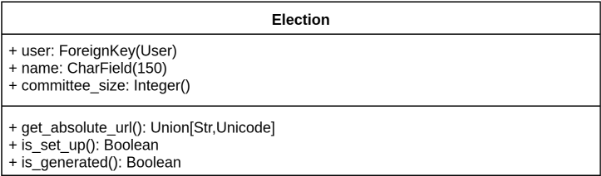
\includegraphics[scale=0.85]{pics/Election.png}}
\captionof{figure}{Obiekt mapowany na tabelę wyborów}
\end{center}
Pola:
\begin{itemize}
\item $user$ - użytkownik aplikacji
\item $name$ - nazwa wyborów
\item $committee\_size$ - rozmiar zwycięskiego komitetu
\end{itemize}
Metody:
\begin{itemize}
\item $get\_absolute\_url()$ - zwraca adres URL, który daje dostęp do danych wyborów z
poziomu dokumentu $.html$
\item $is\_set\_up()$ - zwraca prawdę jeśli dla danych wyborów zostali określeni kandydaci i
głosujący lub fałsz w przeciwnym przypadku
\end{itemize}

\subsection{Candidate}
\begin{center}
\centerline{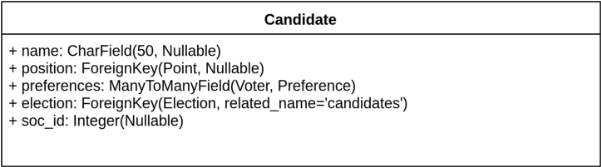
\includegraphics[scale=0.85]{pics/Candidate.png}}
\captionof{figure}{Obiekt mapowany na tabelę z danymi kandydata}
\end{center}
Pola:
\begin{itemize}
\item $name$ - nazwa kandydata
\item $position$ - położenie kandydata w układzie współrzędnych, pole opcjonalne dla
kandydatów generowanych z rozkładu normalnego
\item $preferences$ - pole mapowane na relację wiele do wielu łączącej kandydata i
głosującego w tabeli $Preference$
\item $election$ - wybory, do których należy kandydat
\item $soc\_id$ - identyfikator kandydata w odpowiadającym wyborom pliku w formacie $.soc$,
pole opcjonalne dla wyborów parsowanych z pliku
\end{itemize}

\subsection{Voter}
\begin{center}
\centerline{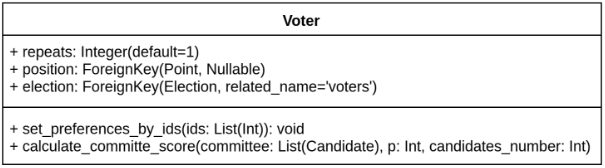
\includegraphics[scale=0.85]{pics/Voter.png}}
\captionof{figure}{Obiekt reprezentujący głos w wyborach}
\end{center}
Pola:
\begin{itemize}
\item $repeats$ - liczba powtórzeń głosów w wyborach
\item $position$ - współrzędne wyborcy na wykresie, pole opcjonalne dla wyborów
generowanych z rozkładu normalnego
\item $election$ - wybory, do których należy głosujący
\end{itemize}
Metody:
\begin{itemize}
\item $set\_preferences\_by\_ids()$ - metoda wykorzystywana przy parsowaniu plików
w formacie $.soc$.
Na podstawie ciągu identyfikatorów wyborców pobranego z pliku tworzy ciąg kandydatów ułożony według preferencji wyborcy. Pobrane dane zapisuje w bazie
danych w postaci rekordu w tabeli $Preference$.
\item $calculate\_committe\_score(committee: List(Candidate), \ p: Int, \
candidates\_number: Int)$ - oblicza wynik komitetu $committee$ na podstawie
parametru $p$ i liczby kandydatów $candidates\_number$. Wynik mnożony jest przez
liczbę powtórzeń głosu.
\end{itemize}

\subsection{Preference}
\begin{center}
\centerline{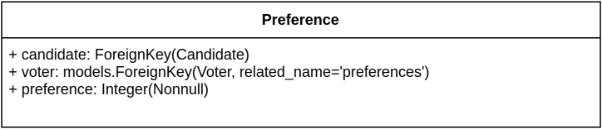
\includegraphics[scale=0.85]{pics/Preference.png}}
\captionof{figure}{Obiekt reprezentujący pozycję kandydata w liście preferencji głosującego}
\end{center}
Pola:
\begin{itemize}
\item $candidate$ - kandydat związany z preferencją
\item $voter$ - głosujący związany z preferencją
\item $preference$ - pozycja preferencji na liście preferencji głosującego 
\end{itemize}

\subsection{Point}
\begin{center}
\centerline{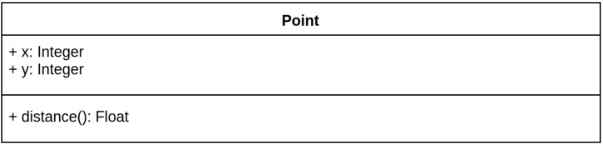
\includegraphics[scale=0.85]{pics/Point.png}}
\captionof{figure}{Obiekt przechowujący współrzędne wyborcy lub kandydata w układzie współrzędnych.}
\end{center}
Pola - współrzędne w układzie kartezjańskim:
\begin{itemize}
\item $x: Int$
\item $y: Int$
\end{itemize}
Metody:
\begin{itemize}
\item $distance(other: Point) : Float$ - metoda zwracająca odległość punktu od punktu $other$ w metryce euklidesowej w przestrzeni $R^2$
\end{itemize}

\subsection{Result}
\begin{center}
\centerline{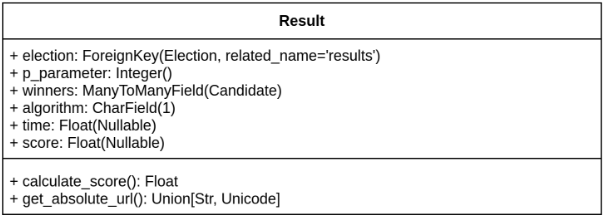
\includegraphics[scale=0.85]{pics/Result.png}}
\captionof{figure}{Obiekt mapowany na tabelę z danymi wyników wyborów: rodzaj algorytmu, parametry
wywołania algorytmu, otrzymany wynik punktowy komitetu oraz czas działania algorytmu}
\end{center}
Pola:
\begin{itemize}
\item $election$ - wybory, dla których obliczono rezultat
\item $p\_parameter$ - parametr $p$ normy $\ell_p$
\item $winners$ - zwycięski komitet
\item $algorithm$ - identyfikator algorytmu
\item $time$ - czas wykonania obliczeń
\item $score$ - wynik punktowy zwycięskiego komitetu
\end{itemize}

\subsection{GeneticAlgorithmSettings}
\begin{center}
\centerline{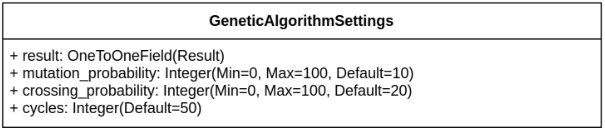
\includegraphics[scale=0.85]{pics/GeneticAlgorithmSettings.png}}
\captionof{figure}{Klasa mapowana na tabelę gromadząca dane specyficzne dla konfiguracji algorytmu
genetycznego. Wykorzystywana do zapisania specyficznych dla algorytmu genetycznego
parametrów wywołania.}
\end{center}
Pola:
\begin{itemize}
\item $result$ - rezultat algorytmu genetycznego
\item $mutation\_probability$ - prawdopodobieństwo wystąpienia mutacji danego osobnika
\item $crossing\_probability$ - prawdopodobieństwo wymiany puli genów pomiędzy parą
osobników
\item $cycles$ - liczba iteracji algorytmu genetycznego
\end{itemize}

\section{Diagram ERD}
\begin{center}
\centerline{\includegraphics[scale=0.45]{pics/ECS_ERD.png}}
\captionof{figure}{Diagram ERD}
\end{center}

\bibliographystyle{alpha}
\bibliography{bibliografia}

\end{document}
